\documentclass[border=2pt]{standalone}

%Drawing
\usepackage{tikz}

\tikzset{>=latex}
\usetikzlibrary{angles, quotes, shapes, decorations.markings, calc}

\tikzstyle{ray} = [postaction=decorate,decoration={markings,mark=at position .52 with \arrow{>}}, red, line width=1.5]
\tikzstyle{gray} = [line width = 1, dashed, black!50]

\newcommand{\point}[4]{
\draw[fill=#4] (#1) circle (2pt) node[#3] {#2};
}

\begin{document}
	
	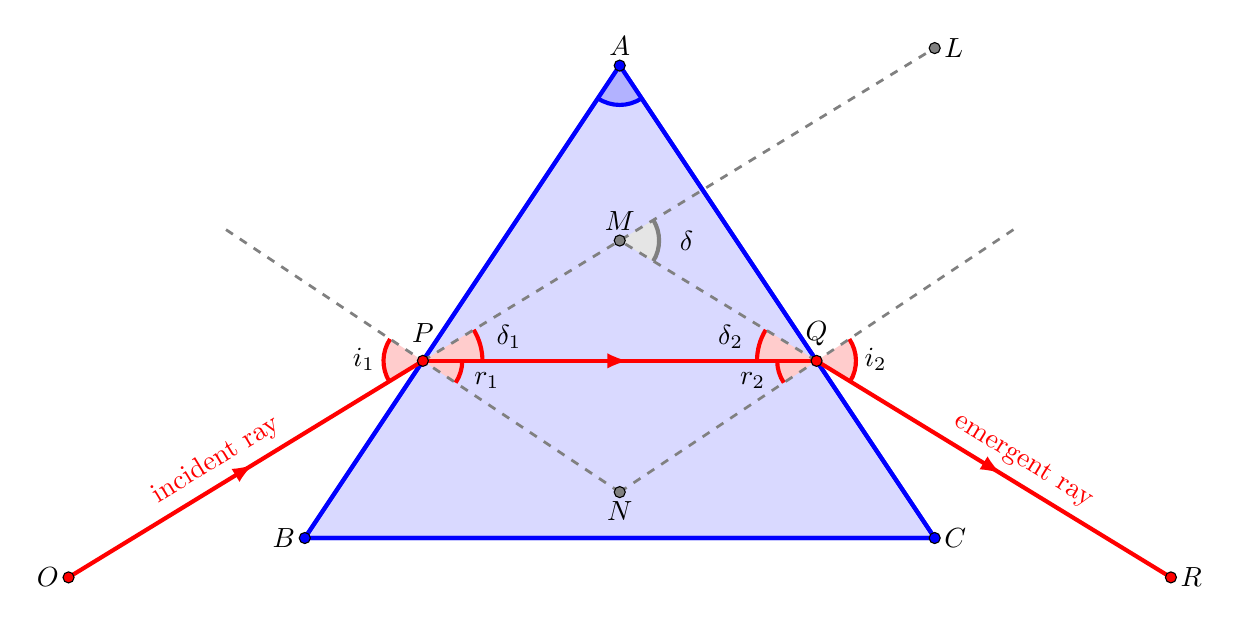
\begin{tikzpicture}
%		% Axis and Grid
%		\foreach \i in {-8,...,0,...,8}
%		{
%			\node at (\i,0) {\i};	
%		}
%		\foreach \i in {-2,...,8}
%		{
%			\node at (0,\i) {\i};	
%		}
		
		% Coordinates
		\coordinate (A) at (0,6);
		\coordinate (B) at (-4,0);
		\coordinate (C) at (4,0);
		\coordinate (O) at (-7,-0.5);
		\coordinate (R) at (7,-0.5);
		\coordinate (P) at (-2.5,2.25);
		\coordinate (Q) at (2.5,2.25);
		\coordinate (N) at (0, 7/12);
		\coordinate (K) at (-5,47/12);
		\coordinate (K') at (5,47/12);
		\coordinate (M) at (0,34/9);
		\coordinate (L) at (4,56/9); 
		
		% Triangle
		\path[draw=blue, fill=blue!15, line width = 1.5] (B) -- (A) -- (C) -- (B); 
		\pic[draw=blue, fill=blue!30, line width=1.5, angle eccentricity=1.5] {angle = B--A--C};
		\draw[line width = 1.5, blue] (B) -- (A) -- (C) -- (B);
		
		% Angles
		\pic[draw=red, fill=red!20, line width=1.5, "$i_1$", angle eccentricity=1.5] {angle = K--P--O};
		\pic[draw=red, fill=red!20, line width=1.5, "$i_2$", angle eccentricity=1.5] {angle = R--Q--K'};
		\pic[draw=red, fill=red!20, line width=1.5, "$r_1$", angle eccentricity=1.7] {angle = N--P--Q};
		\pic[draw=red, fill=red!20, line width=1.5, "$r_2$", angle eccentricity=1.7] {angle = P--Q--N};
		\pic[draw=red, fill=red!20, line width=1.5, "$\delta_1$", angle eccentricity=1.5, angle radius=5ex] {angle = Q--P--M};
		\pic[draw=red, fill=red!20, line width=1.5, "$\delta_2$", angle eccentricity=1.5, angle radius=5ex] {angle = M--Q--P};
		\pic[draw=black!50, fill=black!10, line width=1.5, "$\delta$", angle eccentricity=1.7] {angle = Q--M--L};
		
		% Rays
		\draw[ray] (O) -- (P) node[pos=0.45, sloped, above] {incident ray};
		\draw[ray] (P) -- (Q);
		\draw[ray] (Q) -- (R) node[pos=0.55, sloped, above] {emergent ray};
		
		% Gray Lines
		\draw[gray] (N) -- (K);
		\draw[gray] (N) -- (K');
		\draw[gray] (P) -- (L);
		\draw[gray] (Q) -- (M);
		
		% Points
		\point{R}{$R$}{right}{red}
		\point{Q}{}{above right}{red}
		\point{P}{}{above}{red}
		\point{O}{$O$}{left}{red}
		\point{A}{$A$}{above}{blue}
		\point{B}{$B$}{left}{blue}
		\point{C}{$C$}{right}{blue}
		\point{N}{$N$}{below}{black!50}
		\point{M}{$M$}{above}{black!50}
		\point{L}{$L$}{right}{black!50}
		
		% Nodes
		\node at (-2.5,2.6) {$P$};
		\node at (2.5,2.6) {$Q$};
	\end{tikzpicture}
	
\end{document}